\documentclass{article}
\usepackage{color}
\usepackage{amsmath}
\usepackage{tikz}
\usetikzlibrary{shapes.geometric}
\usetikzlibrary{arrows}
\usetikzlibrary{fit}
\usetikzlibrary{calc}

\newcommand{\bX}{\mathbf X}

\newcommand{\by}{\mathbf y}

\begin{document}

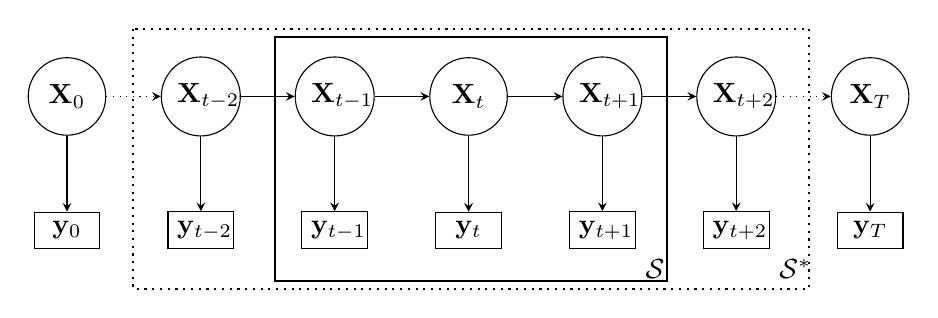
\begin{tikzpicture}[auto=false, node distance=1.7cm]
% Define styles for nodes and arrows
\tikzstyle{latent} = [circle, draw, fill=white, text width=0.6cm, text centered];
\tikzstyle{observed} = [rectangle, draw, fill=white, text width=0.6cm, text centered];
\tikzstyle{arrow} = [->, >=stealth];


% Draw the latent states
\node[latent] (X1) {$\bX_0$};
\node[latent, right of=X1] (X2) {$\bX_{t-2}$};
\node[latent, right of=X2] (X3) {$\bX_{t-1}$};
\node[latent, right of=X3] (X4) {$\bX_t$};
\node[latent, right of=X4] (X5) {$\bX_{t+1}$};
\node[latent, right of=X5] (X6) {$\bX_{t+2}$};
\node[latent, right of=X6] (XT) {$\bX_T$};

% Draw the observed states
\node[observed, below of=X1] (O1) {$\by_0$};
\node[observed, below of=X2] (O2) {$\by_{t-2}$};
\node[observed, below of=X3] (O3) {$\by_{t-1}$};
\node[observed, below of=X4] (O4) {$\by_t$};
\node[observed, below of=X5, label=south east:$\mathcal{S}$] (O5) {$\by_{t+1}$};
\node[observed, below of=X6, label=south east:$\mathcal{S}^*$] (O6) {$\by_{t+2}$};
\node[observed, below of=XT] (OT) {$\by_T$};


\draw[arrow,dotted] (X1) -- (X2);
\draw[arrow] (X2) -- (X3);
\draw[arrow] (X3) -- (X4);
\draw[arrow] (X4) -- (X5);
\draw[arrow] (X5) -- (X6);
\draw[arrow,dotted] (X6) -- (XT);


\draw[arrow] (X1) -- (O1);
\draw[arrow] (X2) -- (O2);
\draw[arrow] (X3) -- (O3);
\draw[arrow] (X4) -- (O4);
\draw[arrow] (X5) -- (O5);
\draw[arrow] (X6) -- (O6);
\draw[arrow] (XT) -- (OT);

\draw[thick] ($(X3.north west)+(-0.4,0.4)$)  rectangle ($(O5.south east)+(0.4,-0.4)$);
\draw[thick,dotted] ($(X2.north west)+(-0.5,0.5)$)  rectangle ($(O6.south east)+(0.5,-0.5)$);


\end{tikzpicture}

\end{document}